\documentclass[uplatex,a4j,11pt,dvipdfmx]{jsarticle}
\usepackage{listings,jvlisting}
\bibliographystyle{junsrt}

\usepackage{url}

\usepackage{graphicx}
\usepackage{gnuplot-lua-tikz}
\usepackage{pgfplots}
\usepackage{tikz}
\usepackage{amsmath,amsfonts,amssymb}
\usepackage{bm}
\usepackage{siunitx}

\makeatletter
\def\fgcaption{\def\@captype{figure}\caption}
\makeatother
\newcommand{\setsections}[3]{
\setcounter{section}{#1}
\setcounter{subsection}{#2}
\setcounter{subsubsection}{#3}
}
\newcommand{\mfig}[3][width=15cm]{
\begin{center}
\includegraphics[#1]{#2}
\fgcaption{#3 \label{fig:#2}}
\end{center}
}
\newcommand{\gnu}[2]{
\begin{figure}[hptb]
\begin{center}
\input{#2}
\caption{#1}
\label{fig:#2}
\end{center}
\end{figure}
}

\begin{document}
\title{レーザー物理学 レポート No.12}
\author{82311971 佐々木良輔}
\date{}
\maketitle
\section*{問20}
簡単のため以下では$\Omega_0^2=y$とする.また$B=C$とする.このとき与式は部分分数分解を行うと
\begin{align}
  \begin{split}
    dt&=\frac{1+By}{A(1-By)y}dy\\
    &=\frac{1}{A}\left(\frac{1}{y}+\frac{2B}{1-By}\right)dy
  \end{split}
\end{align}
となるので.両辺積分し
\begin{align}
  {\everymath{\displaystyle}
  \begin{array}{cl}
    &\int dt=\int\frac{1}{A}\left(\frac{1}{y}+\frac{2B}{1-By}\right)dy\\
    \iff&t=\frac{1}{A}\left(\log y-2\log(1-By)\right)+C\qquad(Cは積分定数)\\
    \iff&At=\log\left(\frac{y}{(1-By)^2}\right)+C\\
    \iff&e^{At}=\frac{Cy}{(1-By)^2}\\
    \iff&0=e^{At}B^2y^2-y(2Be^{At}+C)+e^{At}\\
    \iff&y=\Omega_0^2=\frac{2Be^{At}+C\pm\sqrt{C^2+4BCe^{At}}}{2B^2e^{At}}
  \end{array}
  }
\end{align}
を得る.ここで$B=1/\gamma_1\gamma_2$であったので$B>0$である.また$C=0$においては$y=1/B$と一定値を取るため,立ち上がりの挙動としては不適である.
また$C<0$のとき$y$が実数解を持つ条件は
\begin{align}
  {\everymath{\displaystyle}
  \begin{array}{cl}
    &C(C+4Be^{At})\geq0\\
    \iff&C+4Be^{At}\leq0\\
    \iff&\frac{-C}{4B}\geq e^{At}\\
    \iff&\log\left(\frac{-C}{4B}\right)\geq At
  \end{array}
  }
\end{align}
である.ここで等号が成立する際には
\begin{align}
  \begin{split}
    y&=\frac{2B\frac{-C}{4B}+C\pm\sqrt{C^2+4BC\frac{-C}{4B}}}{2B^2\frac{-C}{4B}}\\
    &=-\frac{1}{B}<0
  \end{split}
\end{align}
であり,光強度が負となる.以上から$C>0$とするべきである.

ここで$C=B=1>0$の場合のグラフは図のようになる.ただし$A=1>0$とした.紫線は$\sqrt{C^2+4BCe^{At}}$の前の符号を正とした場合,赤線は符号を負とした場合である.
この図から符号を正とした場合は$t\rightarrow-\infty$で$\Omega_0^2\rightarrow\infty$であり,立ち上がりの挙動としては不適である.
符号を負とした場合は光強度が$0$から一定の値へと立ち上がることがわかる.

一方で$A<0$とした場合は時間発展を逆向きにすることになるため,紫線は$t\rightarrow\infty$で$\Omega_0^2\rightarrow\infty$となり,
赤線は$t\rightarrow\infty$で$\Omega_0^2\rightarrow0$となるため共に不適である.
\begin{center}
  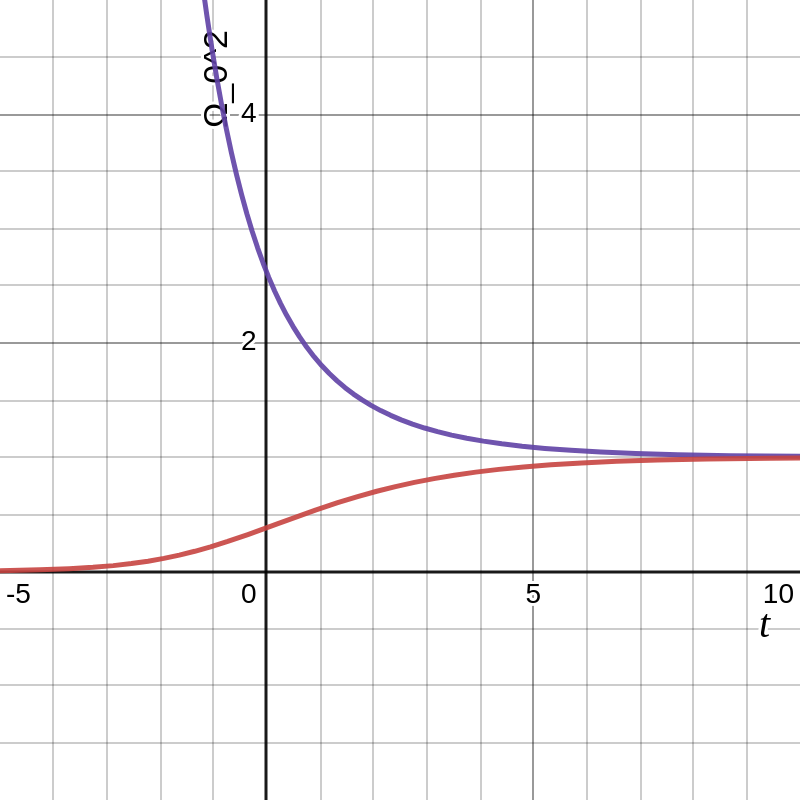
\includegraphics[width=8cm]{desmos-graph.png}
  \fgcaption{$A=B=C=1$のときのグラフ,紫線は符号を正とした場合,赤線は符号を負とした場合}
\end{center}
\section*{問21}
$f(\omega)$を以下で定義する.
\begin{align}
  f(\omega)=\sum_n\delta\left(\omega-\frac{2n\pi}{t_r}\right)
\end{align}
これは周期$2\pi/t_r$の周期関数であり,フーリエ級数展開を用いて
\begin{align}
  f(\omega)=\sum_n\tilde{f}_ne^{in\omega t_r}
\end{align}
と表される.
$\tilde{f}_n$はフーリエ係数であり
\begin{align}
  \begin{split}
    \tilde{f}_n&=\frac{t_r}{2\pi}\int_{-\pi/t_r}^{\pi/t_r}f(\omega)e^{-in\omega t_r}d\omega\\
    &=\frac{t_r}{2\pi}\int_{-\pi/t_r}^{\pi/t_r}\sum_k\delta\left(\omega-\frac{2k\pi}{t_r}\right)e^{-in\omega t_r}d\omega
  \end{split}
\end{align}
ここで積分区間$[-\pi/t_r,\pi/t_r]$には$k=0$の項しか含まれないため
\begin{align}
  \begin{split}
    \tilde{f}_n&=\frac{t_r}{2\pi}\int_{-\pi/t_r}^{\pi/t_r}\delta\left(\omega\right)e^{-in\omega t_r}d\omega\\
    &=\frac{t_r}{2\pi}
  \end{split}
\end{align}
したがって
\begin{align}
  \begin{array}{cc}
    &f(\omega)=\displaystyle\sum_n\cfrac{t_r}{2\pi}e^{in\omega t_r}=\displaystyle\sum_n\delta\left(\omega-\frac{2n\pi}{t_r}\right)\\
    \iff&\displaystyle\sum_ne^{in\omega t_r}=\cfrac{2\pi}{t_r}\displaystyle\sum_n\delta\left(\omega-\frac{2n\pi}{t_r}\right)
  \end{array}
\end{align}
が示される.
\end{document}